% =====================================================================
%  Chapter 5 — The Mathematics, Part III
% =====================================================================

\chapter{The Method, As Its Author Describes It}
\label{ch:method}

This chapter reconstructs the method from the remark's twenty-item timeline.
It is the closest thing available to a proof sketch, and it is a sketch in the
author's own words --- the remark says so itself, calling it ``a rough timeline
Claude provided'' and warning that the parts the author does not personally
understand are ``sort of paraphrasing a `slop' summary, which might make zero
sense.''

What follows is therefore a description of a \emph{described} method. Where the
remark is explicit, this book quotes it. Where it is compressed, this book says
so and marks the reconstruction. And where the timeline's structure reveals
something the remark does not state --- which happens twice --- this book says
that too.

\section{The shape of the twenty items}

The timeline runs from 6 October to 16 November 2026. Sorted by date, it reads:

\begin{center}
\begin{tabularx}{\textwidth}{@{}lX@{}}
\toprule
\textbf{Date} & \textbf{Entry} \\
\midrule
6 Oct & Stepanov determinant\idx{Stepanov determinant} \\
6 Oct & $W(1S) \ge 0$ via a determinant, interpreted as Stepanov with multiplicity one again; ``bootstrap!!'' \\
6 Oct & Iwasawa tower by analogy to pigeonholing on $\FF_{q^n}/\FF_q$ \\
6 Oct & Bost slope inequality\idx{Bost's slope method} \\
8 Oct & $W_1(0,1] + (\sim X\eta)\cdot 1_{(0,1/X]} \ge 0$ gives $> 1-\eta$ \\
9 Oct & $Dp \equiv 0$ on a CM curve for $p$ inert in $K$ \\
14 Oct & Determinants for $W(\cdot)$ containing the desired periods, with GGP periods and interlacing weights \\
14 Oct & Relative trace formula\idx{relative trace formula}; sixfold cover of GL$_5$; automorphy of $\mu$; Cauchy--Schwarz on a projected Poincar\'e series \\
19 Oct+ & $qN = Mk + R\idx{qN = Mk + R}$ using $x_1x_2 + \cdots + x_{k-1}x_k$ \\
20 Oct & Switch to $\Lambda$: $\sum_{n\le X}\Lambda(n)\cdot(X/n-1)_+ - X\log X + (1+\gamma)X$; ``Guinand--Weil\idx{Guinand--Weil sign} had the sign'' \\
15 Nov & Iterated theta lifts\idx{theta lift:iterated} $U(X_0)\to\cdots\to U(X_m)$, winning multiplicity $m$; time to take $m$ like $\sqrt X$ \\
15 Nov & Norms of the lifts, level, cancellation of order-$m$ terms via Chowla--Selberg, Weyl, Siegel mass \\
15 Nov & Sufficient lower bound on divisibility of the $m$-fold iterated lift \\
15 Nov & Rallis seesaw\idx{Rallis seesaw}: the period of the iterated lift is a Bessel period independent of the Hecke characters \\
15 Nov & Precise computation of the ``cost'' of each lift: would stop at 2/3 a priori \\
15 Nov & Glue an integral structure across Hecke characters for a ``gcd'', extra averaging \\
15 Nov & $H^1_o$ classes not killed by twisting: fight for a significant weakening of Vandiver \\
15 Nov & Covolumes, theta series' index, congruences between lifts and forms \\
19 Oct & Precise choice of the Iwasawa tower, specifically using Behrend\idx{Behrend construction} \\
16 Nov & GRH \\
\bottomrule
\end{tabularx}
\end{center}

Two structural features of this table are worth naming.

\begin{quote}
\textbf{It is not chronological.} It is organised by \emph{idea}, with dates
attached. The Stepanov determinant (6 Oct) and the Rallis seesaw (15 Nov) are
twenty months of work apart, but they belong to the same step. The author says
as much: a ``trusted mathematician'' suggested he produce a timeline, and he
produced one organised by the ideas rather than by the days.

\textbf{It has a long silence.} Between 20 October and 15 November there are
five entries, all on 15 November. Whatever happened in those four weeks is not
in the remark. That is the fortnight in which the two-thirds ceiling was
computed and, presumably, addressed.
\end{quote}

\section{Step one: the sign-only Weil bound}

The earliest entries are about producing a positivity statement.

Entry 1 is ``Stepanov determinant'': a determinant whose non-negativity encodes
the desired Weil-type inequality. Entry 4 is the payoff: ``$W(1S) \ge 0$ via a
determinant, interpret as Stepanov with multiplicity one again; bootstrap!!''

This connects directly to the remark's narrative about Stepanov. A determinant
is non-negative exactly when it is a sum of squares, and a sum of squares is
exactly what a Weil positivity argument produces. So ``the sign-only proof of
Weil and Deligne'' mentioned in the remark's page 2 is not a vague gesture: it
is a concrete program --- find a determinant, show it is a Gram matrix, get a
positivity statement for the Weil expression $W$.

And the Weil expression $W$ is the right target, because of Chapter~3's
discussion: Weil's criterion for RH \emph{is} the positivity of the Weil
expression. A method that produces $W \ge 0$ has, if the construction is
faithful, proved RH.

Entry 6 makes the positivity quantitative: ``$W_1(0,1] + (\sim X\eta)\cdot
1_{(0,1/X]} \ge 0$ gives $> 1 - \eta$.'' And entry 7 gives the algebraic
machinery: ``Determinants for $W(\cdot)$'s containing the desired periods,
indeed GGP periods, with values 0, 1 meaning interlacing weights, or up to $m$
non-interlacing ones.''

The vocabulary here is precise and belongs to real research: GGP periods
(Gross--Prasad periods), interlacing weights, and the relation between the two
is a live subject in the theory of automorphic forms. This is not the
vocabulary of a hallucination.

\section{Step two: the divisibility engine}

Entries 2, 3, 5 and 9 form the arithmetic core.

Entry 2 is the CM-curve divisibility: for a prime $p$ inert in $K$ and $D$ the
invariant derivation on the corresponding CM curve, the quantity
$D^a\theta(0)/\Omega^a$ is divisible by $p^{a/p + a/p^3 + \cdots - O(\log a)}$.
This is a Siegel--Ramanujan-type divisibility statement, the kind of thing that
shows up in the theory of Hilbert modular forms and elliptic curves.

Entry 3 is the key algebraic identity: ``$qN = Mk + R$, using $x_1\cdot x_2 +
\cdots + x_{k-1}x_k$, wanting `automorphy' of $N$ since $\mu$ is automorphic
from $\theta$ on sixfold cover of GL$_5$ as a period integral of thetas,
quadric has natural interpretation on corresponding CM e.g.\ $\CC/\ZZ[\omega]$ as
Weil, put Poincar\'e bundle on the edges to get $\theta$s.''

And entry 5 is the moment the method changes gear:

\begin{quote}
\small
``definitively switch to $\Lambda$ aka $\sum_{n \le X}\Lambda(n)\cdot (X/n -
1)_+ - X\log X + (1+\gamma)\cdot X$; Guinand--Weil had the sign, variance test
function trick to $\sum_{h,x_1,\dots,x_k} t(x_1)\cdots t(x_k)\,e_q(h(x_1x_2 +
\cdots + x_{k-1}x_k))$, sum over $h$ first for the left-hand side, with
e.g.\ quadric coefficients too Bertini gives a definite sign from middle
cohomology, one off the one on $M_k$, which is the zero-mode on the right-hand
side with $R$ square-root-quality up to an inch or so as Katz would say by
iterating Parseval $k$ times, opposite signs meaning no cancellation of inverse
roots, QED; vectorize to go up dimensions.''
\end{quote}

This is the most compressed passage in the remark and it is the one where the
author explicitly disclaims understanding (``which might make zero sense, and
I apologize'').

Its content, as far as it can be read, is: the Weil positivity statement is
converted into an estimate for the von Mangoldt sum, via the test-function
trick; the identity $qN = Mk + R$ is the algebraic form of the same positivity
with $M$ a main term and $R$ a remainder; and the ``square-root-quality'' of
$R$ is what makes the final argument work.

The structure is recognisable: this is the classical shape of an analytic
argument for the Weil bound --- a positivity statement, a Fourier transform, a
main term plus a remainder, and a square-root error.

\section{Step three: the lift chain}

Entry 8 is the structural heart of the method:

\begin{quote}
\small
``Iterated theta lifts $U(X_0) \to U(X_1) \to \cdots \to U(X_m)$ between totally
definite unitary groups, $\pi \mapsto \pi \boxplus \mu_j[t]$, wins multiplicity
$m$. Time to take $m$ like $\sqrt X$.''
\end{quote}

\begin{figure}[!htbp]
\centering
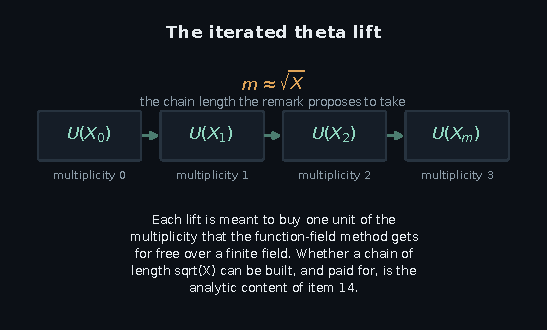
\includegraphics[width=\textwidth]{../figures/fig_theta_lift.pdf}
\caption{The iterated theta lift as the remark describes it. Each lift is
supposed to buy one unit of the multiplicity that the function-field method
gets from the geometry and cannot get over the integers. The remark proposes a
chain of length roughly $\sqrt X$.}
\label{fig:theta-lift}
\end{figure}

The idea, stated plainly, is this. The Stepanov method needs multiplicity. Over
a finite field, multiplicity is free. Over the integers, it is not. But a
theta lift has a feature that behaves like multiplicity: it raises the
dimension of the space of lifts, and, says the remark, it ``wins multiplicity
$m$'' after $m$ iterations. If a chain of length $m$ can be built, then
$m$ units of the missing multiplicity are available.

The remark's own framing of the difficulty, from page 1, is the one-line
summary that the author offers to ``make fellow mathematicians fall out of their
chairs'':

\begin{quote}
\small
``for the von Mangoldt sum of length $X$, Claude's suggested $\sqrt{\ }$ length
of chain of theta lifts, in view of each mimicking multiplicity, was $X$. (And
yet, what else could it be?)''
\end{quote}

The parenthesis is doing a lot of work. It is the sound of an author who finds
the arithmetic coincidence compelling and cannot account for it.

Entries 9, 10, 12, 15 and 18 are the supporting machinery: norms of the lifts
and their level; cancellation of order-$m$ terms via Chowla--Selberg, Weyl and
Siegel mass; a sufficient lower bound on the divisibility of the $m$-fold
iterated lift; the Rallis seesaw, which makes the period of the iterated lift a
Bessel period independent of the Hecke characters; an integral structure glued
across Hecke characters to get a ``gcd'' and extra averaging; and finally the
congruences between lifts and forms.

The Rallis seesaw deserves a note, because it is the single most classical
ingredient in the list. The seesaw identity is the standard mechanism in
automorphic forms by which a period integral on one group is related to one on
another, and it is what makes the ``Bessel period independent of the Hecke
characters'' possible --- that independence is what allows the argument to
average over characters, which is what supplies the missing dimension.

\section{Step four: the automorphy and the tower}

Entries 11, 16 and 19 supply the cohomological and geometric apparatus.

Entry 11: ``Iwasawa tower via analogy\idx{Iwasawa tower} to pigeonhole on $\FF_{q^n}/\FF_q$.''
This is the classical Behrend idea --- a tower of curves over finite fields
whose rational points are controlled, used to manufacture the arithmetic
direction that the integers lack. Entry 19 makes it specific: ``precise choice
of the Iwasawa tower, specifically using Behrend!!'' The double exclamation
appears also in the remark's page 2, where the author describes the moment he
saw ``multiplicity 2 on $O(2,n)$ via the `natively-automorphic' determinant''
and says ``we were going to win but I was also, so to speak, out of my
element, in that I personally have little mastery of automorphic forms on
higher rank groups (youthful foolish stubbornness).''

Entry 16 is the relative trace formula step, and it is the one that connects
the arithmetic analysis to the automorphic side: ``Relative trace formula, seen
in a different half-plane argument via sixfold cover of GL$_5$ automorphy of
$\mu$ and reducing via Cauchy--Schwartz to a bound on the norm of a suitably
projected Poincar\'e series, approximate orthogonality of the columns of the
integral structure.''

\begin{deeper}{How the pieces fit, and where the seam is}
Stated at the highest level of abstraction, the proposed method is:

\begin{enumerate}
\item Produce a \textbf{positivity} statement for the Weil expression, via a
determinant that is a Gram matrix (entries 1, 4, 6, 7).
\item Produce an \textbf{arithmetic divisibility} statement from CM curves and
the identity $qN = Mk + R$ (entries 2, 3, 5).
\item Use \textbf{iterated theta lifts} to manufacture the \textbf{multiplicity}
that the finite-field method gets for free, at a cost of one third of the
multiplicity per lift (entries 8, 9, 10).
\item Use the \textbf{Rallis seesaw} and the \textbf{integral structure} to
average over characters and recover the missing dimension (entries 12, 15, 18).
\item Use the \textbf{relative trace formula} and the \textbf{automorphy of
$\mu$} to make the analytic estimates legitimate, and an \textbf{Iwasawa tower}
to supply the arithmetic growth (entries 11, 16, 19).
\item \textbf{Kill the surviving cohomology} by twisting, which is where
Vandiver enters (entry 17).
\end{enumerate}

The seam is at step 3 combined with step 6: if the cost of each lift is one
third of the multiplicity it buys, and if the twisting does not kill
everything, then the method's natural output is a bound covering two thirds of
the zeros. That is exactly what item 14 computes.

The remark lists, in the same entry, the three things that would be needed to
cross the seam: ``attempt to get a main term and transfer constant to a
function field or kill via twisting, need for `division'.'' Note that all three
are phrased as attempts, and note that the third --- ``division'' --- is the
one that does not appear anywhere else in the twenty items.
\end{deeper}

\section{What the remark never explains}

Three things are conspicuously absent from the remark, and their absence is
more informative than their presence would be.

\begin{enumerate}
\item \textbf{No statement of what is proved.} There is no theorem, no
conjecture numbered 1, and no definition of the objects. The remark's
footnote~4 concedes that it is lossily compressed.
\item \textbf{No explanation of the 15-to-16 November transition.} Item 14
records a ceiling at two thirds; item 20 records GRH. The remark does not
mention the transition.
\item \textbf{No treatment of what ``2/3'' means.} Is it two thirds of the
zeros by count, by multiplicity, simple zeros, or something else? The remark
does not say, and the answer matters, because the known two-thirds theorem of
August 2026 is a statement about zeros that are \emph{simple and on the line}.
\end{enumerate}

\begin{keytakeaways}

\item The method has four stages: a sign-only Weil positivity statement, an
arithmetic divisibility engine based on CM curves and the identity
$qN = Mk + R$, an iterated theta-lift chain supplying the missing multiplicity,
and the automorphic/cocycle apparatus (relative trace formula, Rallis seesaw,
Iwasawa tower) needed to make the estimates legitimate.
\item The vocabulary throughout is that of genuine research --- GGP periods,
interlacing weights, Chowla--Selberg, Siegel mass, Rallis seesaw, Bost's
slope method --- and the dates span six weeks of intensive work.
\item The remark explicitly disclaims the authority of its own summary, and
disclaims the author's understanding of the parts he did not personally
develop.
\item The remark does not explain how the two-thirds ceiling of 15 November
was crossed on 16 November. That is the central open question of this book,
and it is a question about the artifact, because the remark says the Lean
``should suffice to clarify everything''.
\end{keytakeaways}
